\documentclass[oneside]{report}
\usepackage[T1]{fontenc}
\usepackage[utf8]{inputenc}
\usepackage[french]{babel}
\usepackage{graphicx}
\usepackage[margin=2cm]{geometry}
\usepackage{fancyhdr}
\usepackage{changepage}
\usepackage{etoolbox}
\usepackage{xcolor}
\usepackage{listings}
\usepackage{titlesec}
\usepackage{tabu}

\titleformat{\chapter}[display]
{\normalfont\huge\bfseries}{}{20pt}{\Huge}

\titlespacing*{\chapter}{0pt}{0pt}{0pt}
\graphicspath{{./images/}}

\author{Sylvain COMBRAQUE, Sarah LAMOTTE, Nathan JANCZEWSKI, Léo BERGEROT}

\newcommand\softname{Alohomora\ }
\newcommand{\writecol}[1]{
	\subitem{\textcolor[HTML]{#1}{\# #1}}
}

\patchcmd{\chapter}{plain}{fancy}{}{}


\lstset{
	string=[s]{"}{"},
	stringstyle=\color{blue},
	comment=[l]{:},
	commentstyle=\color{black},
}

\begin{document}

	\begin{titlepage}
		\centering
		
\includegraphics[scale=.5]{logo_large}
		\vspace{5cm}
		{\par\scshape\Huge Documents techniques\par}
		\vspace{5cm}
		{\par Gestionnaire de mot de passes\par}
		{\par Application et API\par}
		\vfill
		\par Contact:
		{\par\small Mr.\ Jerôme CUTRONA \par}
		\par jerome.cutrona@univ-reims.fr\
	\end{titlepage}

	\pagestyle{fancy}
	\fancyhf{}
	\lhead{Documents techniques}
	\rhead{
\includegraphics[scale=.25]{logo_large}}
	\tableofcontents

	\chapter{Informations générales}
	\vspace{2cm}
	\par Les requêtes auront lieu à l'URL "https://alohomora.pw/api/". L'API étant basé sur GraphQL, aucune autre route ne sera à prévoir.\\
	\par Le serveur pourra au choix activer ou désactiver l'inscription publique (N'importe qui peut s'inscrire), l'inscription via API (L'utilisateur ne pourra s'inscrire que depuis le site web), le nombre de requêtes par minutes (éviter un flood de 'getUpdates').\\

	\par Les réponses sont envoyé par le serveur au format json.\\

	\chapter{Diagrammes réseau}
	\vspace{2cm}
	\section{Inscription}{
		\par L'inscription au serveur est effectué via une requête register.\\
		\vspace{.5cm}
		\begin{center}
			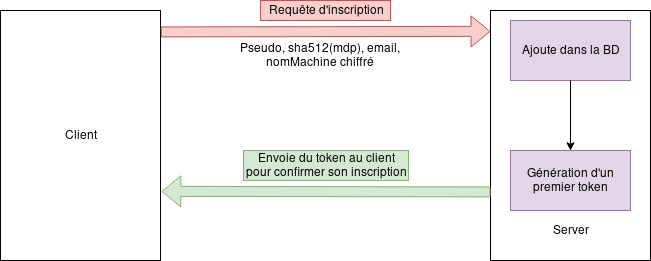
\includegraphics[scale=.5]{reseau_register}
		\end{center}
	}

	\section{Connexion}{
		\par La connexion au serveur permet à l'utilisateur d'obtenir un token lui permettant d'intéragir avec son compte sans que le mot de passe transite. Ce token pourra aussi être révoqué.\\
		\par Lors de la connexion, le client doit générer un couple clé publique / privé OpenPGP. La clé publique est envoyée durant la connexion afin que le serveur puisse reconnaître le client. Cela permettra par la suite la signature des messages.
		\vspace{.5cm}
		\begin{center}
			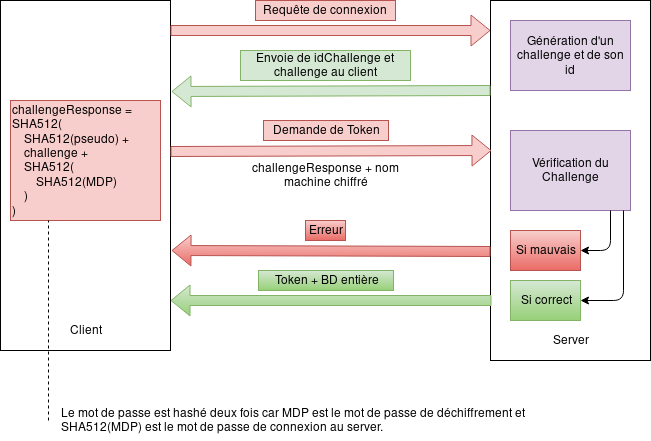
\includegraphics[scale=.5]{reseau_connexion}
		\end{center}
	}

	\section{Récupérer les changements côté serveur}{
		\par Le client peut demander au serveur tous ce qui a changé sur son compte depuis sa dernière mise à jour.
		\par Par défaut, le client peut demander à un interval régulier des mises à jour, cependant le serveur peut refuser et demander au client une synchronisation manuelle via un bouton "Refresh"
		\begin{center}
			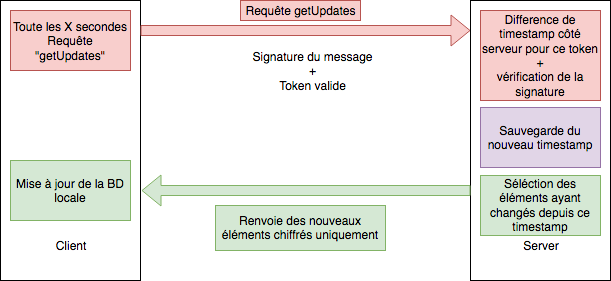
\includegraphics[scale=.5]{reseau_getupdates}
		\end{center}
	}

	\section{Ajout d'un élément}{
		\par Pour ajouter un élément, le client fait une requête en joignant un élément JSON chiffré.
		\par Afin de respecter une cohérence entre les clients, un schéma nécessaire est fourni dans les chapitres suivant de ce document.
		\begin{center}
			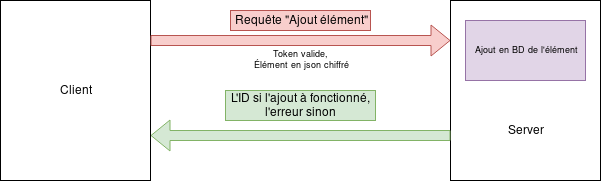
\includegraphics[scale=.5]{reseau_add_elt}
		\end{center}

	}

	\section{Modification ou suppression d'un élément}{
		\par De la même façon que pour ajouter un élément, un client peut le modifier en renvoyant ce dernier et en précisant son ID.
		\par Pour supprimer un élément, le client envoie une requête de modification sans paramètre du contenu.
		\begin{center}
			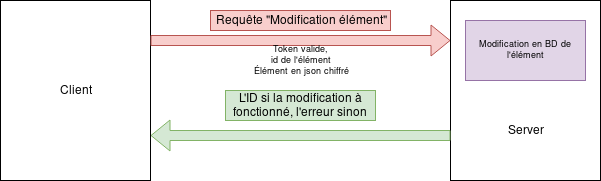
\includegraphics[scale=.5]{reseau_update_elt}
		\end{center}
	}

	\chapter{Client(s)}
	\section{Structuration des données}{
		\subsection{Contenu d'un élément} {
			\vspace{1cm}
			\begin{lstlisting}
				{
					"type": 0,
					"id": 1,
					"name": "Name of the element which will be displayed",
					"customField": { value: "value", hidden: false },
					"customField2": { value: "value", hidden: true }
				}
			\end{lstlisting}
			\vspace{1cm}
			\par Le champ type peut prendre les valeurs 0 dans le cas d'un élément de type "Mot de passe", 1 dans le cas d'un élément de type "Mémo" et 2 dans le cas d'un élément de type "Marque-page". Si la valeur du type est -1.
			\par L'id est un identifiant afin que le client puisse effectuer des requêtes tels que la modification sur un élément.
			\par Le champ nom est le texte affiché quand on souhaite séléctionner un élément afin que l'utilisateur puisse l'identifier.
			\par Après ces champs, dans le cas d'un mot de passe, les autres champs disponibles sont "username", "password" et "url".
			\par Dans le cas d'un mémo le seul champ supplémentaire est un champ "Contenu" qui contiendra le texte du mémo écrite en Markdown.
			\par Enfin, dans le cas d'un marque page, le champ supplémentaire sera "url"
			\par Cependant, des champs personnalisés (Ici représenté par "customfield" et "customfield2") seront ajoutable par l'utilisateur. Il n'y a pas de limite au nombre de champs, l'interface devant donc s'y adapter. Hidden implique que la valeur du champ doit être caché.
		}
	}
	\section{Sécurité}{
		\begin{itemize}
			\item Lors de l'affichage d'une fiche de mot de passe, il ne doit être visible que si l'utilisateur intéragit avec la textfield.
			\item Un bouton permettant de copier le mot de passe doit être mis à disposition afin que l'utilisateur n'ai pas à afficher son mot de passe obligatoirement.
			\item Afin de ne pas pouvoir déduire la longueur du mot de passe, quand il n'est pas affiché une taille fixe pour tous les mots de passes sera utilisée.
			\item Lors du changement de mot de passe, tous les tokens de l'utilisateur sont supprimés.
			\item Un mail peut être envoyé à la connexion d'un utilisateur.
		\end{itemize}
	}

	\section{Ergonomie}{
		\begin{itemize}
			\item Raccourcis clavier CTRL+C / CTRL+B pour copier le mot de passe ou le nom d'utilisateur
		\end{itemize}
	}

	\chapter{Serveur}
	\section{Configuration}{
		\par Un assistant d'installation devra-être créé.
		\begin{itemize}
			\item Autoriser ou interdir l'inscription.
			\item Le serveur peut demander au client de ne pas effectuer des requêtes à interval fixe, dans ce cas, une limite peut être fixée afin de bloquer les requêtes pour éviter le DoS.
		\end{itemize}
	}

	\chapter{Envoie de requêtes}
	\section{Endpoints}{
		\par Liste des endpoints
		\par
		\begin{tabu} to \textwidth {|X|X|X|X|X|}
			\hline
			Endpoint & Méthode & Description & Permissions & Paramètres \\
			\hline
			/users & GET & Liste des utilisateurs & Administrateur & - \\
			- & PUT & Inscription d'un utilisateur & Config & - \\
			- & POST & Login & Tous le monde & - \\
			- & DELETE & Suppression d'un utilisateur & Administrateur & - \\
			- & PATCH & Édition d'un utilisateur & Administrateur & - \\
			\hline
			/token & DELETE & Révoquer un token & Utilisateur du token & - \\
			\hline
			/challenge & GET & Générer un challenge & Tous le monde & - \\
			\hline
			/config & GET & Obtenir la configuration du serveur & Administrateur & - \\
			- & PUT & Sauvegarder la nouvelle configuration & Administrateur & - \\
			\hline
			/element | /groupe & POST & Ajout & Utilisateur & -\\
			- & PUT & Modification & Utilisateur & -\\
			- & DELETE & Suppression & Utilisateur & -\\
			\hline
			/update & GET & Obtenir les éléments changés depuis la dernière requête & Utilisateur & - \\
			\hline
		\end{tabu}
	}

	\section{Création d'une requête}{
		\par Lors de la création d'une requête, à l'exception de Register, Login et Challenge, le client doit spécifier trois header.
		\begin{itemize}
			\item X-ALOHOMORA-TOKEN: Il correspond au token d'authentification de l'utilisateur et de la machine.
			\item X-ALOHOMORA-SIGNATURE: Signature du message pour la clé publique associée au token
			\item User-Agent: Client utilisé pour accéder au service.
		\end{itemize}

		\par L'User-Agent du client officiel est "Alohomora-Client/{OS}", où OS est PC, IOS ou ANDROID.
		\par Le corps de la requête devra contenir un numéro de requête unique au token. Cela permet donc d'éviter les attaques de type Replay. En effet, le serveur sait le numéro de la dernière requête et peut aussi vérifier la signature de la requête.
	}

\end{document}
